\documentclass[UTF8,a4paper,10pt,nocolorlinks]{ctexart}
\usepackage[left=2.50cm, right=2.50cm, top=2.50cm, bottom=2.50cm]{geometry} %页边距
\CTEXsetup[format={\Large\bfseries}]{section} %设置章标题居左   

% 章节标题居中
\usepackage{titlesec}
% \titleformat*{\section}{\centering}
% \titleformat{\section}{\centering\Large\bfseries}{第\,\thesection\,章}{1em}{}
% \titleformat{\section}{\Large\bfseries}{第\,\thesection\,章}{1em}{}
% \makeatletter
% \renewcommand\section{\@startsection{section}{1}{\z@}%
%     % {}%
%     % {-3.5ex \@plus -1ex \@minus -.2ex}%
%     % {2.3ex \@plus.2ex}%
%     {\centering}%
%     {\normalfont\normalsize\CJKfamily{hei}}}
% \makeatother

\usepackage{stfloats}

\usepackage{setspace}
\usepackage{xcolor}
\usepackage{mdframed}
\usepackage{titletoc}
\usepackage{etoolbox}
%%%%%%%%%%%%%%%%%%%%%%%
% -- text font --
% compile using Xelatex
%%%%%%%%%%%%%%%%%%%%%%%
% -- 中文字体 --
%\setmainfont{Microsoft YaHei}  % 微软雅黑
%\setmainfont{YouYuan}  % 幼圆    
%\setmainfont{NSimSun}  % 新宋体
%\setmainfont{KaiTi}    % 楷体
%\setmainfont{SimSun}   % 宋体
%\setmainfont{SimHei}   % 黑体
% -- 英文字体 --
%\usepackage{times}
%\usepackage{mathpazo}
%\usepackage{fourier}
%\usepackage{charter}
\usepackage{helvet}
\usepackage{caption}
\usepackage{multicol} %用于实现在同一页中实现不同的分栏
\usepackage{changepage}
\usepackage{graphics}
\usepackage{amsmath, amsfonts, amssymb} % math equations, symbols
\usepackage[english]{babel}
\usepackage{color}      % color content
\usepackage{graphicx}   % import figures
\usepackage{url}        % hyperlinks
\usepackage{bm}         % bold type for equations
\usepackage{multirow}
\usepackage{booktabs}
\usepackage{epstopdf}
\usepackage{epsfig}
\usepackage{algorithm}
\usepackage{algorithmic}
\newcommand{\sihao}{\fontsize{14pt}{\baselineskip}}
\renewcommand{\algorithmicrequire}{ \textbf{Input:}}     % use Input in the format of Algorithm  
\renewcommand{\algorithmicensure}{ \textbf{Initialize:}} % use Initialize in the format of Algorithm  
\renewcommand{\algorithmicreturn}{ \textbf{Output:}}     % use Output in the format of Algorithm  
\renewcommand{\figurename}{图}

\newcommand{\upcite}[1]{\textsuperscript{\textsuperscript{\cite{#1}}}}

\usepackage{color}
\usepackage{subfigure}
\usepackage{changepage}
\usepackage{fancyhdr} %设置页眉、页脚
\pagestyle{fancy}  %%%单线页眉
\fancyhead{}
\fancyhead[LO]{\emph{Machine Learning Algorithm \& Computer Vision}}
\fancyhead[RO]{\emph{fengxuewei}}

\fancypagestyle{plain}{%
  \pagestyle{fancy}
}
\usepackage{shorttoc}
\usepackage{xcolor}
\usepackage{mdframed}
\usepackage{titletoc}
\renewcommand{\today}{\CJKnumber\year 年 \CJKnumber\month 月 \CJKnumber\day 日}

\DeclareRobustCommand{\chuhao}{\fontsize{42pt}{\baselineskip}\selectfont}  % 初号
\DeclareRobustCommand{\xiaochu}{\fontsize{36pt}{\baselineskip}\selectfont} % 小初
\DeclareRobustCommand{\yihao}{\fontsize{26pt}{\baselineskip}\selectfont}   % 一号
\DeclareRobustCommand{\xiaoyi}{\fontsize{24pt}{\baselineskip}\selectfont}  % 小一
\DeclareRobustCommand{\erhao}{\fontsize{22pt}{\baselineskip}\selectfont}   % 二号
\DeclareRobustCommand{\xiaoer}{\fontsize{18pt}{\baselineskip}\selectfont}  % 小二
\DeclareRobustCommand{\sanhao}{\fontsize{16pt}{\baselineskip}\selectfont}  % 三号 
\DeclareRobustCommand{\xiaosan}{\fontsize{15pt}{\baselineskip}\selectfont} % 小三
\DeclareRobustCommand{\sihao}{\fontsize{14pt}{\baselineskip}\selectfont}   % 四号
\DeclareRobustCommand{\xiaosi}{\fontsize{12pt}{\baselineskip}\selectfont}  % 小四
\DeclareRobustCommand{\wuhao}{\fontsize{10.5pt}{\baselineskip}\selectfont} % 五号
\DeclareRobustCommand{\xiaowu}{\fontsize{9pt}{\baselineskip}\selectfont}   % 小五
\DeclareRobustCommand{\liuhao}{\fontsize{7.5pt}{\baselineskip}\selectfont} % 六号
\DeclareRobustCommand{\xiaoliu}{\fontsize{6.5pt}{\baselineskip}\selectfont}% 小六
\DeclareRobustCommand{\qihao}{\fontsize{5.5pt}{\baselineskip}\selectfont}  % 七号

\providecommand{\keywords}[1]{\textbf{\textit{keywords---}} #1}
 
\usepackage{hyperref} %bookmarks

\captionsetup[figure]{labelfont={bf},labelformat={default},labelsep=period,name={图}}

\hypersetup{colorlinks, bookmarks, unicode} %unicode 
 
\title{\textbf{}}
\author{ fengxuewei \thanks{指导老师:王莉} }
\date{\today}
\begin{document}


\begin{figure}[t]
    \parbox[b]{1cm}{
        
\includegraphics[width=\textwidth]{TYUT.jpg}
        }
\end{figure}

    \begin{center}
        \quad \\
        \quad \\
        \heiti \fontsize{45}{17} 课\quad 程\quad 论\quad 文
        \vskip 3.5cm	
        \begin{center}
            \huge{\textbf{机器学习算法在计算机视觉中的应用与研究}}\\
            \emph{\Large{\textbf{Application and Research of Machine Learning Algorithm in Computer Vision}}}\\
        \end{center}
    \end{center}
        \vskip 3.5cm
    \begin{center}
        \songti \fontsize{15}{15}
        \doublespacing
        % \setlength\parindent{12em} % 首行缩进
        \quad
        \sanhao \\
        学\hspace{1cm}  院:\underline{\qquad 软件学院 \quad}

        专\hspace{1cm}  业:\underline{\qquad 软件工程 \quad} 

        学生姓名:\underline{\qquad 冯学伟 \qquad }     

        学\hspace{1cm} 号:\underline{\quad 2019520941\quad}

        指导教师:\underline{\qquad 王\hspace{0.5em}莉 \qquad}
        % \vskip 2cm
        \centering
        \date{2020年6月14日}
        % \end{flushleft}
    \end{center}

\thispagestyle{empty} % 设置当前页 页版式
\clearpage
	\begin{center}
        \begin{center} % 选择一种技术进行研究
            \huge{\textbf{机器学习算法在计算机视觉中的应用与研究}}\\
            \emph{\Large{\textbf{Application and Research of Machine Learning Algorithm in Computer Vision}}}\\     
        \end{center}
    \end{center}
    
    \begin{adjustwidth}{0cm}{0cm}
        % \textbf 加粗
        \emph{\textbf{摘\hspace{0.5em}要:} 随着机器学习和深度学习技术的快速发展,计算机视觉无疑是近年来发展最快的人工智能领域之一。
        本文针对机器学习在计算机视觉处理中的应用进行了简要分析,
        % 
        并着重分析了典型分类算法—随机森林的算法原理.
        % 在最后就机器学习在计算机视觉中的应用前景进行了展望。随机森林是近几年非常热门的分类方法,由于其训练和测试速度快,被许多学者用于图像匹配、动作识别等领域。利用在线的随机森林,能对跟踪目标进行不断学习,以获取目标最新的外观特征,从而及时完善跟踪,以达到最佳的状态。
        }
        \begin{flushleft}
        \emph{{\textbf{关键字:}} 机器学习; 计算机视觉; 人工智能; 目标跟踪; 随机森林 } %“\par在段首,表示另起一行,“\textbf{}”,花括号内的内容加粗显示
        \end{flushleft}
    \end{adjustwidth}
    \begin{adjustwidth}{0cm}{0cm}
        \emph{\textbf{Abstract:}With the rapid development of machine learning and deep learning technology, computer vision is undoubtedly one of the fastest growing areas of artificial intelligence in recent years. This article briefly analyzes the application of machine learning in computer vision processing, and focuses on analyzing the algorithm principle of a typical classification algorithm-random forest.}\par
    \end{adjustwidth}
    \begin{keywords}
        \emph{\noindent Machine Learning, Computer Vision, AI, Target Tracking, Random Forest}
    \end{keywords}
    \setcounter{page}{1}        %从下面开始编页,页脚格式为导言部分设置的格式

    %%%%%%%%%%%%%%%%%%%%%%%% 分栏 %%%%%%%%%%%%%%%%%%
    \begin{multicols}{2}
    % \section{引言}
    计算机视觉是一种基于计算机算法的自动识别图像内容的
领域,它源于 20 世纪 60 年代左右的人工智能和认知神经科学。
50 年后,GM 图像识别仍然难以普及,但图像识别的发展取得了
显着进展。视觉算法已经开始涵盖广泛的受众,尤其是商业上
的成功,包括交互式分割算法。图像检索,人脸识别和人体动作
捕捉。这些领域的成功必须归功于过去 20 年来机器学习的快
速发展。\par 为此本文分别在图像检测领域、图像语义分割领域介绍了机器学习的应用进展,
着重分析了典型分类算法—随机森林的算法原理。随机森林是近几年非常热门的分类方法,
由于其训练和测试速度快,被许多学者用于图像匹配、动作识别等领域。利用在线的随机森林,能对跟踪目标进行不断学习,以获取目标最新的外观特征,从而及时完善跟踪,以达到最佳的状态。

    \section{图像分类和检测}
        物体分类与检测是计算机视觉、模式识别与机器学习领域非常活跃的研究方向。
        物体分类与检测在很多领域得到广泛应用,包括安防领域的人脸识别、行人检测、智能视频分析、行人跟踪等,
        交通领域的交通场景物体识别、车辆计数、逆行检测、车牌检测与识别,以及互联网领域的基于内容的图像检索、相册自动归类等。
        \par 可以说,物体分类与检测已经应用于人们日常生活的方方面面,
        计算机自动分类与检测技术也在一定程度了减轻了人的负担,改变了人类生活方式。
        计算机视觉理论的奠基者,英国神经生理学家马尔认为,视觉要解决的问题可归结为“What is Where”,
        即什么东西在什么地方,即计算机视觉的研究中,物体分类和检测是最基本的研究问题之一。
        比如当我们面对一张图片的时候,最基础的任务就是这张图片是什么,是风景图还是人物图、是描写建筑物的还是关于食物的,
        这就是分类。\par
        分类作为一个较为笼统的目标,还是较为好达成的。当知道了图像的类别的时候,进一步的就是检测了,
        例如我知道这个图像是关于人脸的,那么这个人脸在哪里,能不能把它框出来。检测作为一个较为精细的目标,
        达成的难度可以说是远大于分类的。
    \par 如图\ref{fig1}所示,给定一张图片,物体分类要回答的问题是这张图片中是否包含某类物体(比如牛);物体检测要回答的问题则是物体出现在图中的什么地方,即需要给出物体的外接矩形框,如图\ref{fig1:b}所示。
        \begin{figure*}[htpb]
            \centering
            \subfigure[物体分类] {
                \label{fig1:a}     
                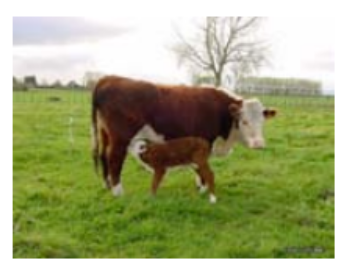
\includegraphics[width=0.45\textwidth]{pictures/row1.png}  
            }     
            \subfigure[物体检测] { 
                \label{fig1:b}     
                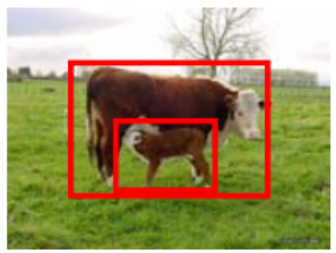
\includegraphics[width=0.45\textwidth]{pictures/row2.png}     
            }    
            \caption{视觉识别}%n张图片共享的说明
            \label{fig1}
        \end{figure*}
        物体分类与检测的研究,是整个计算机视觉研究的基石,是解决跟踪、分割、场景理解等其他复杂视觉问题的基础。
        欲对实际复杂场景进行自动分析与理解,首先就需要确定图像中存在什么物体(分类问题),或者是确定图像中什么位置存在什么物体(检测问题)。
        鉴于物体分类与检测在计算机视觉领域的重要地位,研究鲁棒、准确的物体分类与检测算法,无疑有着重要的理论意义和实际意义。
        广义的目标检测不仅包括物体检测(Object Detection),还包括边缘检测(Border Detection)及关键点检测(Landmark Detection)等。
        \subsection{边缘检测}
        边缘检测,在很多场景下可以看作是图像分割(Segmentation)任务(图像分割的边界往往就是物体的边缘)。
        而图像分割也包括传统算法和深度学习语义分割;
        而目标检测类算法(如R-CNN)也经常延伸到语义分割。
        图像分割与目标检测有着千丝万缕的关系。传统的图像分割主要包括:阈值分割、区域生长、分水岭算法、微分算子法、主动轮廓模型、小波变换等方法。这些传统图像分割方法是计算机视觉的基础知识,具体此处不赘述。其中微分算子法很有启发意义,采用算子(又称“核”、“过滤器”)检测特定模式,启发我们可以通过设计特定的卷积核来检测特定的刚性目标。
        
        \subsection{关键点检测}
        此处将关键点(Landmark、Benchmark)、特征点都称为感兴趣点。
        主要方法包括:Harris角点检测法、SIFT特征点检测法、基于模型的ASM或AAM法、基于级联形状回归CPR,和基于深度学习的算法。
        其中,Harris角点检测法是设计角点检测算子,对图像每个像素都计算响应值,然后确定一个合适的阈值来检测角点。
        基于模型的ASM法,是先对标记点所在的物体形状进行配准对齐,然后通过构建的局部特征,进行局部搜索和匹配;
        AAM法则在ASM法的基础上加了纹理特征。

        \subsection{机器学习与计算机视觉}
        机器学习是研究计算机如何模拟人类学习行为以获取新知
识或技能,并重新组织现有知识结构以不断提高其绩效。它是
人工智能的核心,也是使计算机智能化的根本途径。为了实现计
算机视觉的功能,可以采用两种技术方法,分别是仿生学方法
和工程方法。\par
其中工程学方法的一般做法是将人类视觉系统视为黑盒子,
并且实现仅关注视觉系统将为输入提供何种输出。这两种方法
在理论上都是可用的,但难点在于人类视觉系统对应于某个输
入的输出不能直接测量。而且因为人类智力活动是多功能系统
组合的结果,即使得到输入输出对,也很难确定它是仅由当前输
入视觉刺激产生的响应。 而不是一个与历史状态综合作用的
结果。

    \section{随机森林分类模型}
    在照片\ref{fig1}中,计算机通过算法实现“语义图像分割”,并区分
    三个主要元素:背景,母牛,小牛,这需要一个强大的构建块
    来实现,即训练分类器预测不同分类图像(如树木,天空,人,牛等)中像素的分布。这项任务给机器学习带来了很多计算问
    题,特别是那些包含大量像素的计算机,这意味着我们需要在
    整个图像分类任务中进行超过一百万次的培训和测试。\par
    面对如此大的像素问题,通常使用更有效的分类模型:
随机森林。 随机森林以随机方式建造,构造森林后,当一个新
的输入样本进入时,让森林中的每个决策树分别进行判断。查看
样本应属于哪个类别,然后查看最多选择哪个类别,预测该类
使用哪个样本。这种模型的优势在于:它可以处理许多高维数据,不需要进行特征选择,是一种很好的降维方法;在训练完后,
它能够给出哪些 feature 比较重要;它的训练速度较快;在训练
过程中,可以检测到特征之间的相互影响 ; 容易做成并行化方
法。\par
    \subsection{随机森林使用背景}
        \subsubsection{随机森林定义}
        随机森林顾名思义,
        是一种比较新的机器学习模型。经典的机器学习模型是神经网络,
        有半个多世纪的历史了。神经网络预测精确,但是计算量很大。
        上世纪八十年代Breiman等人发明分类树的算法(Breiman et al. 1984),
        通过反复二分数据进行分类或回归,计算量大大降低。
        2001年Breiman把分类树组合成随机森林(Breiman 2001a),
        即在变量(列)的使用和数据(行)的使用上进行随机化,生成很多分类树,再汇总分类树的结果。\par
        简而言之,随机森林是用随机的方式建立一个森林,森林里面有很多的决策树组成,随机森林的每一棵决策树之间是没有关联的。在得到森林之后,当有一个新的输入样本进入的时候,就让森林中的每一棵决策树分别进行一下判断,看看这个样本应该属于哪一类(对于分类算法),然后看看哪一类被选择最多,就预测这个样本为那一类。
        \subsubsection{随机森林应用范围}
        随机森林主要应用于回归和分类。
        随机森林和使用决策树作为基本分类器的bagging有些类似。以决策树为基本模型的bagging在每次bootstrap放回抽样之后,产生一棵决策树,抽多少样本就生成多少棵树,在生成这些树的时候没有进行更多的干预。而随机森林也是进行bootstrap抽样,但它与bagging的区别是:在生成每棵树的时候,每个节点变量都仅仅在随机选出的少数变量中产生。因此,不但样本是随机的,连每个节点变量(Features)的产生都是随机的。
        许多研究表明, 组合分类器比单一分类器的分类效果好,随机森林(random forest)是一种利用多个分类树对数据进行判别与分类的方法,它在对数据进行分类的同时,还可以给出各个变量(基因)的重要性评分,评估各个变量在分类中所起的作用。
    \subsection{随机森林算法}
    随机森林(RondomFroest, RF)是Leo Breiman结合Bagging集成学习理论和随机子空间方法在
    2001年发表的一种机器学习算法。RF是一种统计学
    习理论,其利用bootstrap重抽样方法从原始样本中抽
    取多个样本,对每个bootsrap样本进行决策树建模,然
    后组合多棵决策树的预测,通过投票得出最终预测结
    果。RF具有分析复杂分类特征的能力,对于噪声数据
    和存在缺失值的数据具有很好的鲁棒性,并具有较快
    的学习速度,其变量重要性度量可作为高维数据的特
    征选择工具,近年来已经被广泛应用于各种分类、预
    测、特征选择以及异常点检测问题中。\par
    \begin{figure}[H]
        \centering % 图片居中
        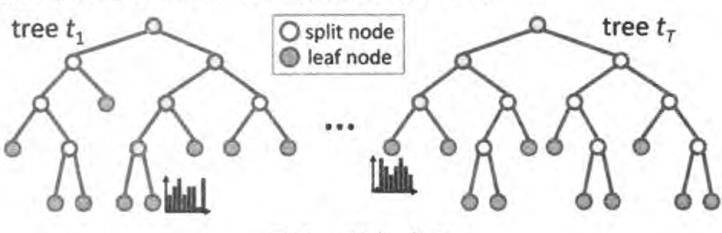
\includegraphics[width=0.4\textwidth]{pictures/RF.png} 
        \caption{随机森林}
        \label{fig:FR}
    \end{figure}
    RF是一个由一组决策树分类器组成的集成分类
    器,如式\ref{equ:1},其中是服从独立同分布的随机向量,K
    表示随机森林中决策树的个数,在给定输入自变量x
    下,每个决策树分类器通过投票来决定最优的分类
    结果
    \begin{equation} % 等式
        \left\{ h(X, \theta_{k}) , k = 1, 2, \dots, K \right\}
        \label{equ:1}
    \end{equation}
    \par RF的构建过程如下:
    \begin{itemize}
        \item[(1)]在给定的原始训练数据集中,利用Bootstrap
        方法有放回的抽取K个样本,且每个样本的样本容量
        都和原始训练数据集相同;
        \item[(2)]利用K个样本集构建K个决策树模型,组合
        成RF模型。
        每颗决策树的构建过程:
            \begin{itemize}
                \item[1)] 在分裂节点$n$,从$m$个样本特征中随机的抽取$m_{try}$个特征($m_{try}$<<$m$)组成节点$n$的特征向量$V$;
                \item[2)] 计算特征向量$y$的一个分裂函数$f$的值,根据随机产生的阈值$t$,将训练数据集 $I_{n}$ 递归的分裂成左
            右两个子集$I_{i}$和$I_{r}$
                \begin{align}
                    & I_{l} = \left\{ i \in I_{n} | f(V_{I}) < t \right\} \\
                    & I_{r} = \frac{I_{n}}{I_{l}}
                    \label{equ:2}
                \end{align}
                \item[3)] 计算根据此分裂函数$f$,和阈值$t$分裂,节点$n$的
                信息增益,信息增益的计算公式如下
                \begin{equation}
                    \triangle E = -\frac{I_{l}}{I_{n}} E(I_{l}) - \frac{\left\| I_{r} \right\|}{\left\| I_{n} \right\|} E(I_{r})
                    \label{equ:4}
                \end{equation}
                其中, E(I)是样本集I的香农熵;
                \item[4)] 因有多个分裂函数$f$和阈值$t$,所以选择产生信
                息增益$\triangle E$最大的那一对分裂函数$f$和阈值$t$进行
                分裂;
                \item[5)] 样本集递归的沿着决策树向下训练,直到到达
                树的最大深度$D$或者不再产生信息增益。
            \end{itemize}
            \item[(3)] 对新的数据进行分类时,分类结果根据K个决策树决策结果来进行投票,得票最多的类别为RF
            决策的结果
            \begin{equation}
                H(x) = argmax_{Y} \sum_{i=1}^k I(h_i (x) = Y)
            \end{equation}
            其中,$H(x)$表示组合分类器模型;$h_{i}$表示单个决策树模型;$Y$表示输出变量;$I(^o)$表示示性函数。上式是使
用投票系统来确定最终分类的原理。
    \end{itemize}
    
    \subsection{基于随机森林的图像语义分割算法}
    在图像分类领域,常采用方法框架是,首先提取感
兴趣的特征点,利用特征点周边信息将特征点量化为
数值向量,这些数值向量被用于模型的学习或分类测
试图像。基于随机森林的像素对比图像语义分割算法
在将特征点量化为数值向量的过程中,直接利用了图
像的低级像素信息(像素值对比),而不是通过计算复
杂的滤波器组相应或局部描述子,在算法速度上,随机
森林在训练和测试均较快,尤其是与k—meas聚类算
法、特征描述子的最近邻赋值算法比较。该算法在训
练阶段,从训练库图像中随机地采样出固定大小的窗
口作为特征,通过窗口中随机的选取的两个像素点的
像素值对比,将这些特征量化为数值向量,这样的向量
集合被用于训练随机森林分类器;在测试阶段,以每个
像素点作为中心,提取一个窗口,在这个窗口中提取一
个向量集合,利用随机森林的叶子节点对这些向量分
别进行投票,根据投票结果选举产生该像素点最可能
的归属类别,通过对整个图像的每一个像素进行类别
预测,可快速的对图像完成语义分割。基于随机
森林的像素对比图像语义分割算法步骤:
    \subsubsection{提取训练图像块}
    从训练集合中采用滑动窗口方法提取出大量的图
像块,如图\ref{pic:block}所示,每个图像块的类别为其中心像素点
在groudtruth中指定的类别.
\begin{equation}
    P = < pathVector, c >
\end{equation}
其中,patchVector表示图像块在颜色空间中的像素值,
如块的宽度为d,则patchVector可表示为 d × d × 3,c
为 groudtruth 中指定的类别。
\begin{figure}[H]
    \centering % 图片居中
    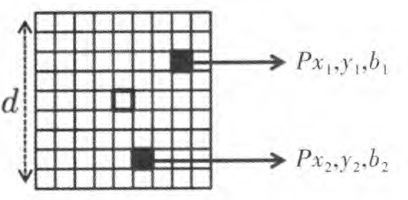
\includegraphics[width=0.4\textwidth]{pictures/pict_block.png} 
    \caption{图像块大小}
    \label{pic:block}
\end{figure}
\subsubsection{计算每个类别的权重}
在一些数据集上,可能有大量的数据明显的偏向
某些特定的类别。因此,在此数据集上学习的分类器
将会相应的偏向这些特定的类别。为了修正这些偏差,文中给每一个训练样本一个相应的权重$\omega_{i}$,权重
为对应样本所属的类别占总样本的频率
\begin{align}
    \omega_{i} &= \xi_{c_{i}} \\
    \xi_{c} &= ( \sum_{i \in I} [ c = c_{i} ] )
\end{align}
利用这些权重训练而来的分类器能更好的决策出
每一个类别。经过训练,文中利用训练数据集,而不
是随机的自己子集$I^{'}$,得到了一个改善的类别分布估
计。可轻微的提升分类器的综合性能,尤其是当数据
集较少时。
\subsubsection{不变性学习}
尽管利用原始的像素值作为特征比计算描述子或
滤波器组响应更快,却导致失去了固有的不变性特征。
为此,采用仿射变换的形式,对训练集合中的图像进行
几何变换和光照变换。通过几何变换和光照变换,可
对特定的问题学习到适当的不变性特征,提升分类器
的分类性能。在实验当中,探索了几何变换中的旋转、
缩放、左右翻转等变换,以及光照仿射变换。

\subsubsection{训练随机森林} 
根据随机森林理论,对提取的图像块数据集进行
训练,在决策树分裂节点$n$处,直接随机选取图像块$P$
上两个像素点$P_{xl,yl,bl}$和$P_{x2,y2,b2}$组成特征向量$V$,如图\ref{pic:block}所示,其中像素($x_1, y_1$)和像素($x_2, y_2$)可能来自不同
的颜色通道$b_{1}$和$b_{2}$。图像块p上,分裂函数$f$有4种
表示方式:(1)单个像素($x, y$)在颜色通道b的值
$P_{x,y,b}$;(2)两个像素的和$P_{xl,yl,bl}$ + $P_{x2,y2,b2}$;(3)两个像
素的差值$P_{xl,yl,bl}$ - $P_{x2,y2,b2}$;(4)两个像素的绝对差值
$|P_{xl,yl,bl} - P_{x2,y2,b2}|$。\par
在RF中,引入随机性,可减少相关性而保持强度
不变,提高预测精度。故在此改进了上述分裂函数$f$
的选取方式,引人随机性,将上面4种分裂方式线性组
合起来,产生一个随机的分裂函数$f$,,如式\ref{equ:5},其中
$\lambda_{1}, \lambda_{2}, \lambda_{3}, \lambda_{4}$随机选取从$-1 \sim 1$的值

\begin{align}
    f = & \lambda_1 P_{x, y, b} + \lambda_2 (P_{x_1, y_1, b_1} + P_{x_2, y_2, b_2}) +  \nonumber \\ 
        & \lambda_3 (P_{x_1, y_1, b_1} - P_{x_2, y_2, b_2}) + \nonumber \\
        & \lambda_4 ( | P_{x_1, y_1, b_1} - P_{x_2, y_2, b_2} | )
    \label{equ:5}
\end{align}
    由于每一个图像块P的特征向量y和分裂函数$f$
的选取都是随机的,相互独立的,当图像块$P$的数量足
够多时,根据数理统计中的中心极限定理可知以,f(V)服
从正态分布N($\mu, \sigma^2$),随机阈值t根据此正太分布随
机产生。根据分裂函数$f$和阈值$t$分裂,计算节点$n$的
信息增益$\Delta E$,选取产生最大信息增益$\Delta E$最大的那一
对分裂函数$f$和阈值$t$进行分裂。样本集递归的沿着
决策树向下训练,直到到达树的最大深度$D$或者不再
产生信息增益。\par
每颗决策树根据以上规则充分的生长,不需要剪
枝,直到训练完所有决策树,组合成随机森林,图\ref{fig:FR}所示。
    \section{结 论}
    计算机视觉的研究是具有双重意义的,首先它是为了满足
    人工智能应用的需求,即需要用计算机实现手动视觉系统,这
    些结果可以安装在计算机和各种计算机上,使计算机和机器人
    能够“看到”。反过来,视觉计算模型的研究成果对于我们进一
    步理解和研究人类视觉系统本身的机制,甚至是人脑的机制具
    有重要的参考意义。本文首先针对机器学习在计算机视觉处理中的
    应用进行了简要分析,分别在图像检测领域、图像语义分割领域
    介绍了机器学习的应用进展,并着重分析了典型分类算法—随
    机森林的算法原理,在最后就基于随机森林的图像语义分割
    的算法进行了叙述。FR算法通过直接利用图像低级的像素信息,而
    不是去计算复杂的滤波器组响应或者局部描述子,可以大
    幅提高了算法训练和测试速度。
    \end{multicols}
    \clearpage % 分页

\addcontentsline{toc}{section}{参考文献}
\renewcommand{\refname}{参考文献}   % 将References改为参考文献
\begin{thebibliography}{99}
\addtolength{\itemsep}{-2ex} % 用于更改行距

\bibitem{1}吴政隆,李杰,关震宇, 等.基于光流的固定翼小型无人机自主着陆控制[J].系统工程与电子技术,2016,38(12):2827-2834. DOI:10.3969/j.issn.1001-506X.2016.12.22.
\bibitem{2}刘浩林.基于视觉的微小型固定翼UAV自主定点降落系统的研究[D].陕西:西安理工大学,2018.
\bibitem{3}刘康.基于Matlab的移动物体检测与识别[D].陕西:西安石油大学,2017.
\bibitem{4}王广彪,李华伟,丁文锐, 等.无人机在运动舰船上着舰视觉导引技术研究[J].中国电子科学研究院学报,2012,7(3):274-278,283. DOI:10.3969/j.issn.1673-5692.2012.03.011.
\bibitem{5}嵇盛育.基于计算机视觉的无人机自主着舰导引技术研究[D].江苏:南京航空航天大学,2008. DOI:10.7666/d.d053499.
\bibitem{6}张棋,陈朝伟,熊锴.机器学习在计算机视觉处理中的应用[J].数码世界,2019,(6):56.
\bibitem{7}章永来,周耀鉴.聚类算法综述[J].计算机应用,2019,39(7):1869-1882. DOI:10.11772/j.issn.1001-9081.2019010174
\bibitem{8}于万霞,张维存,郑宏兴.基于遗传粒子群算法的高维复杂函数优化方法[J].计算机工程与应用,2007,43(36):31-33. DOI:10.3321/j.issn:1002-8331.2007.36.011.
\bibitem{9}李少波,宋启松,李志昂, 等.遗传算法在机器人路径规划中的研究综述[J].科学技术与工程,2020,20(2):423-431.
\bibitem{10}姜勇,姜智,郭鑫, 等.基于遗传算法-反向传播神经网络的地下无人驾驶车辆自主导航技术[J].机械制造,2018,56(12):26-30. DOI:10.3969/j.issn.1000-4998.2018.12.008.
\bibitem{11}郭梓桐. 机器学习算法在计算机视觉领域的应用[J]. 科技经济导刊, 2020, (3):27-28.
\bibitem{12}蒋瀚, 刘怡然, 宋祥福等. 隐私保护机器学习的密码学方法[J]. 电子与信息学报, 2020, (5):1068-1078.
\bibitem{13}Zhang, D., Zuo, W., \& Yue, F. (2012). A Comparative Study of Palmprint Recognition Algorithms. ACM Computing Surveys, 44(1), 1–37. doi:10.1145/2071389.2071391 
\bibitem{14}Galleguillos, C.,\& Belongie, S. (2010). Context based object categorization: A critical survey. Computer Vision and Image Understanding, 114(6), 712–722. doi:10.1016/j.cviu.2010.02.004 
\bibitem{15}Chen, S., Xu, Y., Zhou, X., \& Li, F. (2019). Deep Learning for Multiple Object Tracking: A Survey. IET Computer Vision. doi:10.1049/iet-cvi.2018.5598 
\bibitem{16}Ming-Hsuan Yang, Kriegman, D. J., \& Ahuja, N. (2002). Detecting faces in images: a survey. IEEE Transactions on Pattern Analysis and Machine Intelligence, 24(1), 34–58. doi:10.1109/34.982883 
\bibitem{17}张万福.基于随机森林的图像语义分割算法的研究[J].电子科技,2017,30(2):72-75. DOI:10.16180/j.cnki.issn1007-7820.2017.02.019.
\bibitem{18}张友鹏.一种基于光流的行人阴影检测与跟踪[J].现代计算机,2019,(8):53-57. DOI:10.3969/j.issn.1007-1423.2019.08.011.
\bibitem{19}马越.实时人眼定位算法的研究与实现[D].上海:上海交通大学,2016.
\bibitem{20}鲁帅.视频监控中目标检测与跟踪算法研究[D].上海:复旦大学,2012.
\end{thebibliography}  

\end{document}